%!TEX root = cscw2018-comic.tex
\section{Discussion}
\label{sec:Discussion}
Our experiment answers RQ-1 affirmatively in that comics are more persuasive than text, with a moderate effect of 0.33. Our answer to RQ-2 while the effect of no element is significant, shading and gesture show strong influence, but surprisingly inter-character distance is most effective when distance is large. For RQ-3, we show that negative messages are more influential than positive messages. We have developed a prototypical comic generator (answering RQ-4) that can be used in deploying comic messages.

Next we discuss the question of inter-character distance, followed by a discussion of color in comics. We conclude this section with a discussion of study limitations.

%

% Next we discuss the question of inter-character distance, follwoed b Our analysis shows that subjects prefer persuasive messages in comic form over plain text. We found in a persuasive comic, different character's gestures and background shading can influence subjects' perception of the persuasiveness whereas no strong effect was found in inter-character distance. This was consistent with previous research on visual stimulus in persuasion and the benefits of comics in communication.
%
\subsection{Inter-Character Distance}
\label{sub:Inter-Character Distance}
There may be two explanations to the odd result that the farthest distance between the two characters was more influential.

However, previous studies on comics composition suggests the inter-character distance can affect reader's perceived relationship between characters and therefore influence their perception of the persuasive comics.

First, it may be the case that the subjects did not project themselves onto the comic as one of the characters and did not recognize the distance between characters as reflecting closeness of the relationship. For example, a subject may read the comic from a third-person narrative. We looked into some feedbacks from in the pilot study. One participant ($p_1$) mentioned \textit{``I really like the comic I just saw and I feel bad that someone told me ...''} which suggests the subject does think that they are in the comic and having a conversation with someone else. Yet, we don't know if they perceive their relationship with the persuader based on the inter-character distance. A second explanation is that closer inter-character distance causes a cluttered visual composition and thus the subjects perceive these comics as less visually pleasing.

\subsection{Comics with Color}
\begin{figure}[t]
 \centering
 \begin{tabular}{ccc}
  \subfloat[Colored Text]{\label{figur:3o}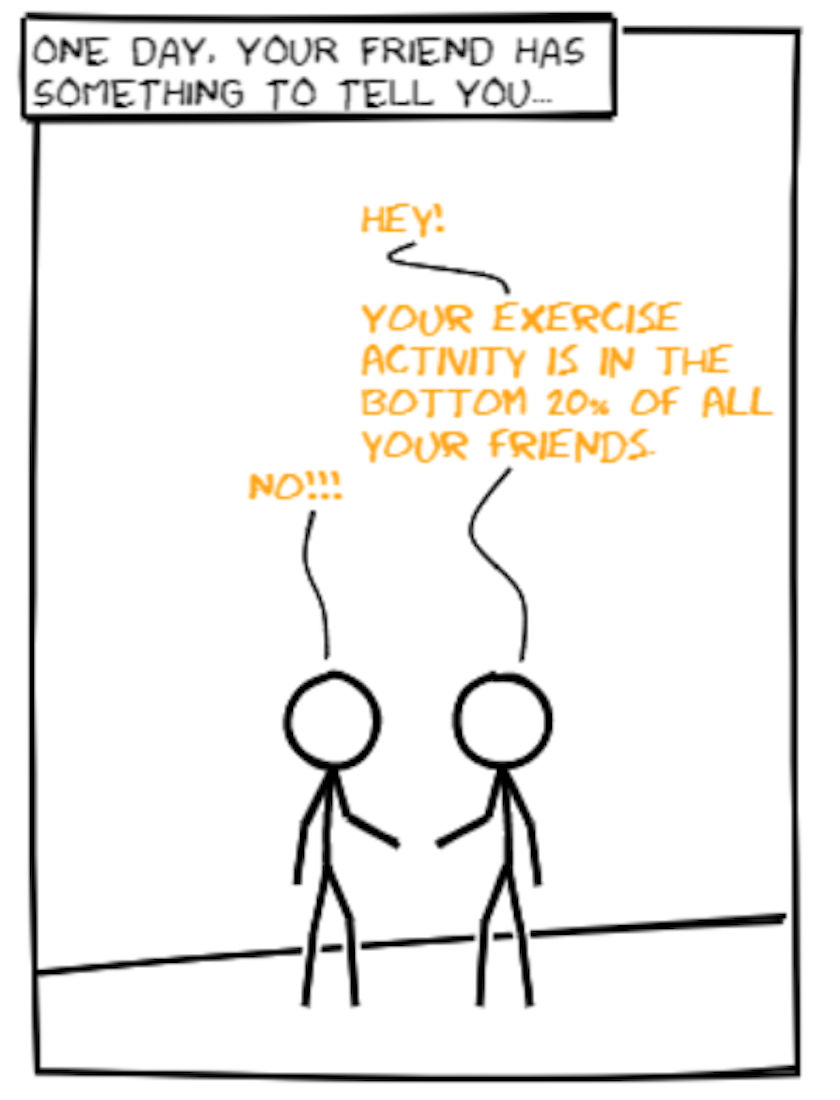
\includegraphics[width = 0.27\columnwidth]{figures/o1}} &
  \subfloat[Colored Ground Line]{\label{figur:31}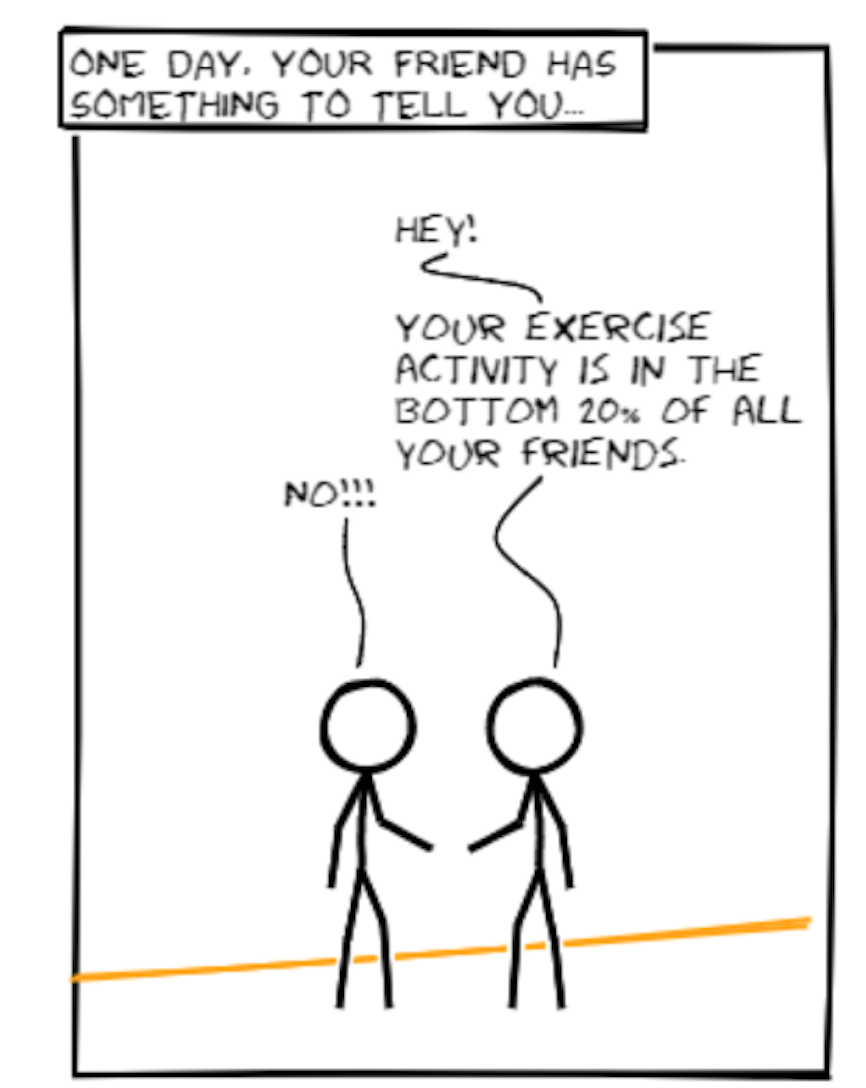
\includegraphics[width = 0.27 \columnwidth]{figures/o2}}      &
  \subfloat[Colored Figure]{\label{figur:32}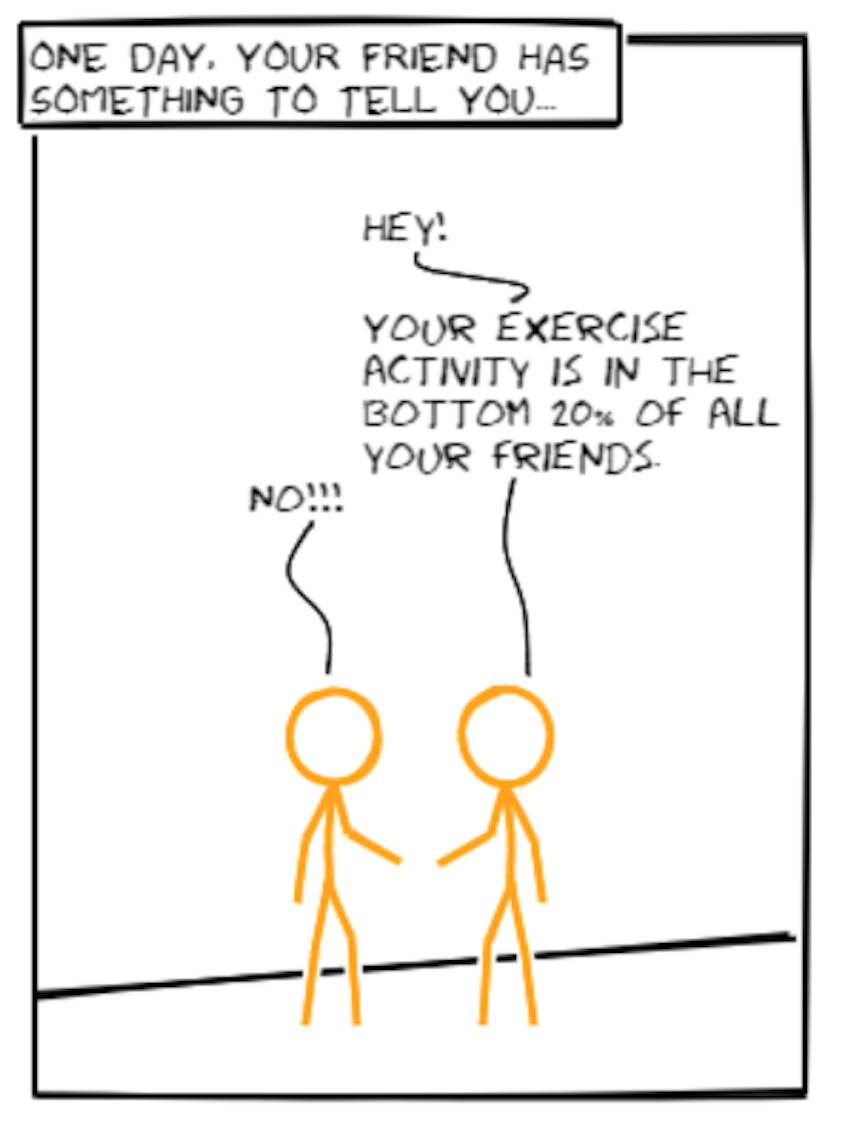
\includegraphics[width = 0.27 \columnwidth]{figures/o3}}\\
 \end{tabular}
 \caption{Colored different elements in a comic}
 \label{figur:color}
\end{figure}

Our model suggests the background shading in a persuasive comic affects its persuasive power which makes us wonder the role of color as previous studies suggest the usage of color communicates the emotional intensity similar to the background shading. We ran a small scale study comparing the perceived persuasiveness between black-white comics in our study and their corresponding colored version,see figure~\ref{figur:color}. With 60 participants from the Mechanical Turk,  we found using an identical hierarchical Bayesian formulation that our subjects perceive colored version as more persuasive and there is potential interaction effect between negative-positive framing and different colors (see~\Cref{fig:color-experiment-effect}). We plan to run larger experiments that include color and study the interaction with framing and other elements.

\begin{figure}
 \subfloat[The mean effect and the effect size with color\label{subfig-1:color-mean-effect}]{%
  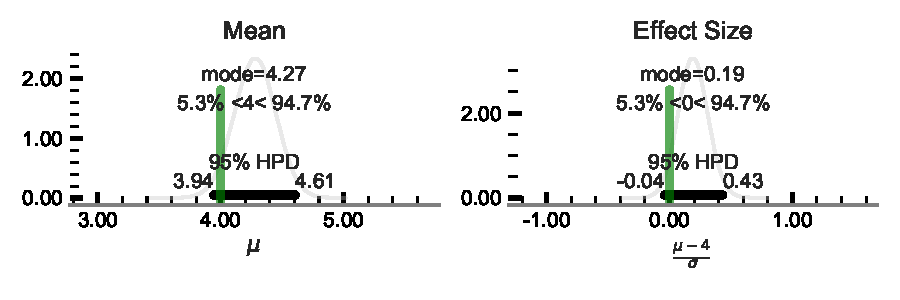
\includegraphics[width=0.6\textwidth]{./hari-code/factors_mean_effect_color-no-interaction.pdf}
  } \hfill
 \subfloat[Color contrast\label{subfig-2:color-contrast}]{%
  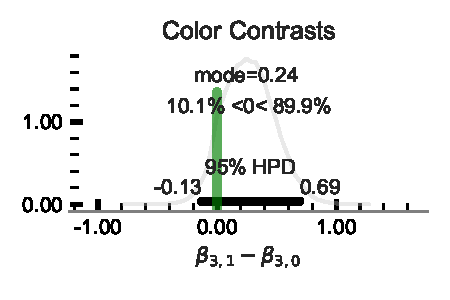
\includegraphics[width=0.33\textwidth]{./hari-code/factors_color_contrasts_color-no-interaction.pdf}
 }
 \caption{~\Cref{subfig-1:color-mean-effect} shows the High Posterior Density (HPD) intervals for the mean response $\mu$ and effect sizes $\sigma_y$ in the presence of color. HPD represent the region with 95\% of the density. Notice that the HPD interval for $\mu$ is $[3.94, 4.27]$ and includes a ROPE of $[4\pm 0.1]$ (the interval includes 4, the neutral response value). Thus while there no significant effect, we note that nearly 94\% of the HPD lies to the right of 0. The figure for effect size shows a small effect with mode $0.19$; since the HPD interval $[-0.04, 0.43]$ includes a ROPE of $[0\pm 0.1]$, there is no significant effect.~\Cref{subfig-2:color-contrast} shows the contrasts between the use of the two colors. The modal value is $0.24$, but since the HPD interval $[-0.13, 0.69]$ overlaps with 0, there is no appreciable effect (but notice that 89\% of the density lies in the region greater than 0.)}
 \label{fig:color-experiment-effect}
\end{figure}

% \subsection{Towards Computational Persuasion}
% Research on computational persuasion identified one of the major challenges as constrained persuasion protocols\cite{huntertowards}. In our study, we created a framework that has the potential to automatically create XKCD style persuasive comics based on the input of conversation texts and a set of parameters and configure three key elements in the comic including character's gesture, inter-character distance, and background shading accordingly. With the integration of computational persuasion model in the future, the framework can synthesize persuadee's personal data to create comics with maximum persuasive power. For example, when persuading a risk-averse individual who values group norm to engage more exercise, a piece of persuasive comic showing a group of his/her friends are talking to the persuadee with negative-framed facts about him/her at a gym can be algorithmically created by our future framework.

\subsection{Limitations}
Our current work has several limitations.
\begin{description}
 \item[Single Panel]: Our experiment limits our comics to a single panel which hinders one of the most fascinating aspect of comics---storytelling. Comparing to the comic strip, single panel comics find it harder to show the dynamic among characters.
 \item[No interaction effects in model]: Our model does not include any interaction effects. This is by design, since we have 54 experimental conditions making the any analysis interaction effects difficult with our small observational study. The raw data suggests an interaction between shading and gesture, but given our limited dataset, there is little point in modeling this interaction. We plan to study interaction effects in future studies by limiting the number of main predictor conditions.
 \item[Generalizability]: We examined a single case---exercise. While the setting of abstract comics appears to be general, without any additional studies on topics such as food, or even the more general case of collective action dilemmas (e.g. reducing carbon footprint), it is unclear how well our framework generalizes. We plan to conduct additional experiments to test these different scenarios.
 \item[Ecological Validity:] There is a ligitimate question if our experiment on Amazon Mechanical Turk has ecological validity, since we ask the subjects (who may lack  interest in exercise) to evaluate persuasiveness when the topic is on exercise. Notice that our goal is not to persuade experimental subjects to exercise more, but to evaluate if the comic is a more persuasive form of communication of a statistical fact. We should expect---since we don't know if the subjects are interested in exercise---an increase in the variance in the estimates of the parameters (in particular,  $\sigma_y$). Despite this, the analysis show a significant affirmative result for RQ-1.
 \item[Appropriate gestures]: The authors determined gestures used by the characters in the experiment through trial and error. It may be useful to examine dance theory as well as work on designing sign languages.
\end{description}

% First, our comics are limited to only single panel which hinders one of the most fascinating aspect of comics, storying telling. Comparing to the comic strip, it is difficult for single panel comics to show the dynamic among characters which can better bring the reader into the comics according to the previous research. Second, although comics can convey meanings for different topics, comics are rarely used in working email and official documents, which suggests comics may be better used for on topic than another. In our study, we only examined the persuasive power of comics in nudging people to exercise. Further investigations for other persuasion topics, such as stopping crime, increasing working efficiency, are needed. Third, in our study, the different levels of those three key elements in the comics are suggested by the authors where the differences among levels are not consistent. As our result suggests, for the gesture and background shading, the effects are strong between neutral and extreme and between neutral and medium but not strong between extreme and medium which suggests potential inequality. In the future, we could have expert cartoonist and experience judges work together to create different levels for each comics elements.
